\documentclass[11pt,a4paper]{article}

% ── Packages ──────────────────────────────────────────────
\usepackage[margin=2.5cm]{geometry}
\usepackage{graphicx}
\usepackage{booktabs}
\usepackage{enumitem}
\usepackage{xcolor}
\usepackage{listings}
\usepackage{hyperref}
\usepackage{amsmath}
\usepackage{tikz}
\usetikzlibrary{arrows.meta, positioning, shapes.geometric, fit, calc}
\usepackage{caption}
\usepackage{subcaption}
\usepackage{fancyhdr}
\usepackage[T1]{fontenc}
\usepackage{lmodern}

% ── Colors ────────────────────────────────────────────────
\definecolor{codebg}{HTML}{1E1E2E}
\definecolor{codetext}{HTML}{CDD6F4}
\definecolor{accent}{HTML}{89B4FA}
\definecolor{green}{HTML}{A6E3A1}
\definecolor{red}{HTML}{F38BA8}
\definecolor{yellow}{HTML}{F9E2AF}
\definecolor{dimtext}{HTML}{6C7086}

% ── Listings ──────────────────────────────────────────────
\lstset{
  language=C++,
  basicstyle=\ttfamily\small\color{codetext},
  backgroundcolor=\color{codebg},
  keywordstyle=\color{accent}\bfseries,
  commentstyle=\color{dimtext}\itshape,
  stringstyle=\color{green},
  numbers=left,
  numberstyle=\tiny\color{dimtext},
  numbersep=8pt,
  frame=single,
  rulecolor=\color{dimtext},
  breaklines=true,
  tabsize=4,
  showstringspaces=false,
  xleftmargin=1.5em,
  framexleftmargin=1.5em,
  morekeywords={override, nullptr, auto, unique_ptr, string, set, pair, vector}
}

% ── Header/Footer ────────────────────────────────────────
\pagestyle{fancy}
\fancyhf{}
\lhead{\small\textit{Gateless Gate --- Erae Shape Editor}}
\rhead{\small\textit{George Redpath}}
\cfoot{\thepage}

% ── Title ─────────────────────────────────────────────────
\title{%
  \vspace{-1cm}
  \textbf{Gateless Gate: Interactive Shape Editing}\\[0.3em]
  \large Right-Click Edit Mode for the Erae Touch~II Layout Editor\\[0.2em]
  \normalsize\textit{Feature Implementation Report --- Thesis Appendix}
}
\author{George Redpath\\[0.2em]
  \small NTNU / Aalborg University}
\date{\today}

% ══════════════════════════════════════════════════════════
\begin{document}
\maketitle
\thispagestyle{fancy}

% ── Abstract ──────────────────────────────────────────────
\begin{abstract}
This document describes the design and implementation of the \textbf{Edit Shape}
mode in the Erae Shape Editor, a JUCE-based visual layout editor for the Erae
Touch~II multi-touch surface. The feature allows users to right-click any
existing shape and interactively modify its geometry through simultaneous
cell painting, erasing, and handle-based resizing---all without mode switching.
Non-pixel shapes (rectangles, circles, hexagons, polygons) are transparently
auto-converted to pixel representations on first edit. The implementation spans
four source files, introduces a new undo action type, and adds a
\texttt{replaceShape()} primitive to the layout model. This work forms part of
the \textit{Gateless Gate} project, a modular Eurorack synthesizer system
combining FPGA-based DSP with touch-based control surfaces.
\end{abstract}

% ══════════════════════════════════════════════════════════
\section{Context: The Gateless Gate Project}

The Gateless Gate is a 104\,HP Eurorack modular synthesizer built around a Zynq-7020
FPGA (Zybo Z7-20 board) containing 302 SystemVerilog DSP modules, 56 audio
channels (28~ADC + 28~DAC), and a patent-pending 1-Wire automatic patch topology
detection system. The project encompasses approximately 116,000 lines of code
across FPGA gateware, embedded firmware, and desktop software.

The \textbf{Erae Shape Editor} serves as a complementary touch-based control
interface. Where the Gateless Gate hardware uses physical rotary encoders and
illuminated jacks, the Erae Touch~II provides a $42 \times 24$ grid multi-touch
surface capable of continuous pressure and position tracking. The editor
application---built as a JUCE VST3/Standalone plugin---lets musicians design
custom touch layouts with shapes, colors, MIDI behaviors, and visual feedback
styles, then push them to the hardware surface over USB SysEx.

\begin{figure}[h]
  \centering
  \includegraphics[width=0.85\textwidth]{screenshot.png}
  \caption{Erae Shape Editor showing a Wicki-Hayden isomorphic keyboard layout
    with 10-finger multitouch tracking, per-finger color palette, and
    real-time hardware rendering.}
  \label{fig:editor}
\end{figure}

% ══════════════════════════════════════════════════════════
\section{Motivation}

Prior to this work, the editor supported five shape types---Rectangle, Circle,
Hexagon, Polygon, and Pixel---each created through dedicated drawing tools.
However, \textbf{modifying an existing shape's geometry} required deleting it and
redrawing from scratch, losing all associated behavior configuration (MIDI
mappings, velocity curves, visual style, z-ordering).

Musicians frequently need to fine-tune shape boundaries: adjusting pad sizes by
a pixel or two, carving notches for adjacent shapes, or adding extensions to
irregular freeform layouts. The lack of in-place editing was a significant
workflow friction point.

The solution is an \textbf{Edit Shape} mode that provides three simultaneous
editing actions without mode switching:
\begin{enumerate}[nosep]
  \item \textbf{Paint} cells onto the shape (left-click/drag)
  \item \textbf{Erase} cells from the shape (right-click/drag)
  \item \textbf{Resize} via drag handles (corners and edges)
\end{enumerate}

% ══════════════════════════════════════════════════════════
\section{Interaction Design}

\begin{figure}[h]
  \centering
  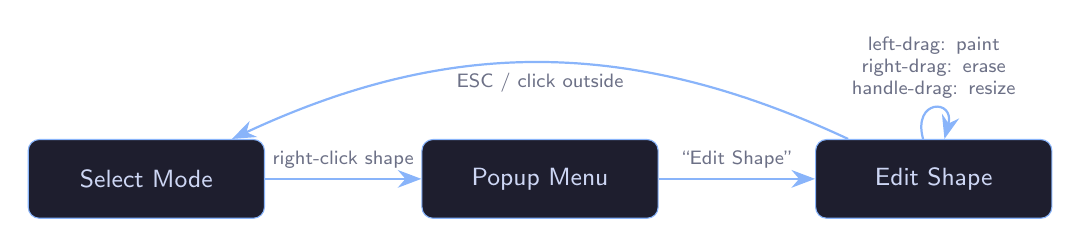
\begin{tikzpicture}[
    state/.style={rectangle, rounded corners=4pt, draw=accent, fill=codebg,
                  text=codetext, minimum width=3cm, minimum height=1cm,
                  font=\small\sffamily},
    action/.style={-{Stealth[length=3mm]}, thick, color=accent},
    label/.style={font=\scriptsize\sffamily, color=dimtext}
  ]
    % States
    \node[state] (select) at (0,0) {Select Mode};
    \node[state] (popup) at (5,0) {Popup Menu};
    \node[state] (edit) at (10,0) {Edit Shape};

    % Transitions
    \draw[action] (select) -- node[above, label] {right-click shape} (popup);
    \draw[action] (popup) -- node[above, label] {``Edit Shape''} (edit);
    \draw[action, bend right=25] (edit) to node[below, label] {ESC / click outside} (select);

    % Self-loops for edit actions
    \draw[action, loop above, looseness=5] (edit) to
      node[above, label, text width=3cm, align=center] {left-drag: paint\\right-drag: erase\\handle-drag: resize} (edit);
  \end{tikzpicture}
  \caption{State transition diagram for the Edit Shape interaction.}
  \label{fig:states}
\end{figure}

The interaction flow is:

\begin{enumerate}
  \item In \textbf{Select mode}, the user right-clicks a shape. A context menu
        appears with a single option: \textit{Edit Shape}.
  \item Selecting it enters \textbf{Edit Shape mode} for that specific shape.
        The canvas displays:
        \begin{itemize}[nosep]
          \item A per-cell grid overlay highlighting every cell belonging to the shape
          \item Eight resize handles (four corners, four edge midpoints)
          \item An ``EDIT SHAPE (ESC to finish)'' indicator
        \end{itemize}
  \item The user modifies the shape freely:
        \begin{itemize}[nosep]
          \item \textbf{Left-click/drag}: adds grid cells to the shape (live update)
          \item \textbf{Right-click/drag}: removes grid cells from the shape (live update)
          \item \textbf{Handle drag}: scales all cells proportionally to fit the new bounding box
        \end{itemize}
  \item \textbf{ESC} or clicking $>3$ cells outside the bounding box commits
        the edit and returns to Select mode.
  \item \textbf{Ctrl+Z} reverses the entire editing session as a single undo step.
\end{enumerate}

% ══════════════════════════════════════════════════════════
\section{Auto-Conversion Strategy}

A key design decision is handling non-pixel shapes. Rectangles, circles,
hexagons, and polygons store geometry parametrically (origin, width/height,
radius, vertex list), not as discrete cells. When the user paints or erases
a single cell, the shape must be converted to a \texttt{PixelShape} to support
arbitrary cell-level editing.

\begin{table}[h]
  \centering
  \caption{Auto-conversion behavior by edit action type.}
  \label{tab:conversion}
  \begin{tabular}{@{}lll@{}}
    \toprule
    \textbf{Action}    & \textbf{Converts to Pixel?} & \textbf{Reason} \\
    \midrule
    Paint cell         & Yes (on first cell edit)     & Cell-level granularity requires pixel storage \\
    Erase cell         & Yes (on first cell edit)     & Removing a cell breaks parametric geometry \\
    Handle resize      & Yes (cells are scaled)       & Scaled cells no longer fit parametric form \\
    \bottomrule
  \end{tabular}
\end{table}

The conversion captures the shape's current \texttt{gridPixels()} output---the
rasterized set of integer grid coordinates---and constructs a
\texttt{PixelShape} with equivalent cells. All visual properties (color, active
color, behavior, behavior parameters, z-order, visual style) are preserved
through the conversion.

Undo reverses the conversion entirely, restoring the original parametric shape.

% ══════════════════════════════════════════════════════════
\section{Architecture}

The implementation touches four files across three layers of the application
architecture:

\begin{figure}[h]
  \centering
  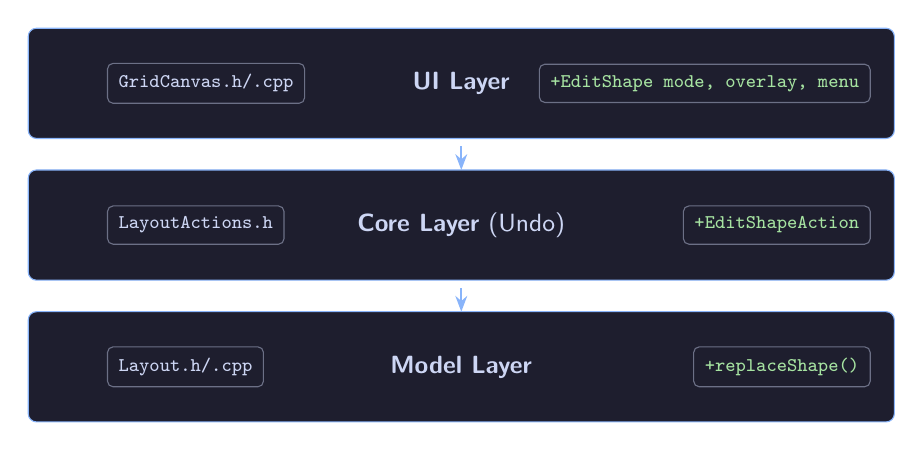
\begin{tikzpicture}[
    layer/.style={rectangle, rounded corners=3pt, draw=accent, fill=codebg,
                  text=codetext, minimum width=11cm, minimum height=1.4cm,
                  font=\small\sffamily},
    file/.style={rectangle, rounded corners=2pt, draw=dimtext, fill=codebg,
                 text=codetext, font=\scriptsize\ttfamily, inner sep=4pt},
    arrow/.style={-{Stealth[length=2mm]}, thick, color=accent}
  ]
    % Layers
    \node[layer] (ui) at (0, 3) {\textbf{UI Layer}};
    \node[layer] (core) at (0, 1.2) {\textbf{Core Layer} (Undo)};
    \node[layer] (model) at (0, -0.6) {\textbf{Model Layer}};

    % Files
    \node[file, anchor=west] at (-4.5, 3) {GridCanvas.h/.cpp};
    \node[file, anchor=west] at (-4.5, 1.2) {LayoutActions.h};
    \node[file, anchor=west] at (-4.5, -0.6) {Layout.h/.cpp};

    % Changes summary (right side)
    \node[file, anchor=east, text=green] at (5.2, 3)
      {+EditShape mode, overlay, menu};
    \node[file, anchor=east, text=green] at (5.2, 1.2)
      {+EditShapeAction};
    \node[file, anchor=east, text=green] at (5.2, -0.6)
      {+replaceShape()};

    % Arrows
    \draw[arrow] (0, 2.2) -- (0, 1.9);
    \draw[arrow] (0, 0.4) -- (0, 0.1);
  \end{tikzpicture}
  \caption{Architectural layers and files modified. Green text indicates additions.}
  \label{fig:arch}
\end{figure}

\subsection{Model Layer: \texttt{Layout.h/.cpp}}

A single new method was added to the \texttt{Layout} class:

\begin{lstlisting}[caption={The replaceShape method preserves z-order position.}]
void Layout::replaceShape(const std::string& id,
                          std::unique_ptr<Shape> newShape)
{
    for (auto& s : shapes_) {
        if (s->id == id) {
            s = std::move(newShape);
            sortByZOrder();
            notifyListeners();
            return;
        }
    }
}
\end{lstlisting}

This swaps a shape in-place by ID, preserving its position in the shape vector
(and thus its z-order after re-sorting). This is preferable to
\texttt{extractShape()} followed by \texttt{addShape()}, which would lose the
shape's position among peers of equal z-order.

\subsection{Core Layer: \texttt{EditShapeAction}}

A new undo action stores cloned copies of both the original and final shape
states:

\begin{lstlisting}[caption={EditShapeAction uses clones for repeatable perform/undo.}]
class EditShapeAction : public UndoableAction {
    Layout& layout_;
    std::string id_;
    std::unique_ptr<Shape> oldShape_;  // clone of original
    std::unique_ptr<Shape> newShape_;  // clone of edited result

    void perform() override {
        layout_.replaceShape(id_, newShape_->clone());
    }
    void undo() override {
        layout_.replaceShape(id_, oldShape_->clone());
    }
};
\end{lstlisting}

Cloning on every perform/undo ensures the action remains valid across multiple
undo/redo cycles. The memory cost is minimal---each \texttt{PixelShape} stores
only a vector of $(x,y)$ integer pairs.

\subsection{UI Layer: \texttt{GridCanvas}}

The bulk of the implementation lives in the canvas component. The
\texttt{ToolMode} enum gains a new value:

\begin{lstlisting}
enum class ToolMode {
    Select, Paint, Erase, DrawRect, DrawCircle,
    DrawHex, DrawPoly, DrawPixel, EditShape
};
\end{lstlisting}

Five new member variables track the editing session:

\begin{table}[h]
  \centering
  \caption{Edit-mode state variables.}
  \label{tab:state}
  \begin{tabular}{@{}llp{7cm}@{}}
    \toprule
    \textbf{Variable} & \textbf{Type} & \textbf{Purpose} \\
    \midrule
    \texttt{editingShapeId\_} & \texttt{string} & ID of the shape being edited (empty = not editing) \\
    \texttt{editOrigShape\_} & \texttt{unique\_ptr<Shape>} & Clone of shape before any edits (for undo) \\
    \texttt{editCells\_} & \texttt{set<pair<int,int>{}>} & Current cell set in absolute grid coordinates \\
    \texttt{editConverted\_} & \texttt{bool} & Whether we auto-converted from a parametric shape \\
    \texttt{editDraggingHandle\_} & \texttt{HandlePos} & Which resize handle is being dragged \\
    \bottomrule
  \end{tabular}
\end{table}

% ══════════════════════════════════════════════════════════
\section{Key Implementation Details}

\subsection{Live Synchronization}

Every paint or erase action immediately synchronizes the in-memory cell set
back to the layout model via \texttt{syncEditCellsToShape()}. This method:

\begin{enumerate}[nosep]
  \item Computes the bounding box origin $(\min x, \min y)$ from \texttt{editCells\_}
  \item Builds relative cell coordinates: $(c_x - \min x,\; c_y - \min y)$
  \item If the shape is not yet a \texttt{PixelShape}, constructs one and calls
        \texttt{replaceShape()}
  \item If already a \texttt{PixelShape}, updates \texttt{relCells} in-place and
        notifies listeners
\end{enumerate}

This provides immediate visual feedback: the shape redraws on every cell
change, and widgets (pressure glow, fill bars) continue to render correctly
because the layout model stays consistent.

\subsection{Handle-Based Scaling}

When the user drags a resize handle, all cells are proportionally scaled to fit
the new bounding box. The algorithm:

\begin{enumerate}[nosep]
  \item Compute the old bounding box $(x_0, y_0, w_0, h_0)$ from current cells
  \item Compute the new bounding box $(x_1, y_1, w_1, h_1)$ from the handle delta
  \item For each cell $(c_x, c_y)$, map to the new box:
        \[
          c'_x = \lfloor x_1 + (c_x - x_0) \cdot w_1 / w_0 \rfloor, \quad
          c'_y = \lfloor y_1 + (c_y - y_0) \cdot h_1 / h_0 \rfloor
        \]
  \item Clamp to grid bounds $(0 \le c' < 42, \; 0 \le c' < 24)$
\end{enumerate}

This produces nearest-neighbor scaling of the cell pattern, which preserves
shape topology while allowing arbitrary aspect ratio changes through all eight
handle positions.

\subsection{Context Menu}

The right-click context menu uses JUCE's asynchronous popup system to avoid
blocking the message thread:

\begin{lstlisting}[caption={Asynchronous popup menu with lambda callback.}]
juce::PopupMenu menu;
menu.addItem(1, "Edit Shape");
menu.showMenuAsync(
    juce::PopupMenu::Options().withTargetScreenArea(
        juce::Rectangle<int>(e.getScreenX(),
                             e.getScreenY(), 1, 1)),
    [this, shapeId](int result) {
        if (result == 1)
            enterEditMode(shapeId);
    });
\end{lstlisting}

The lambda captures the shape ID by value, ensuring correctness even if the
layout changes between menu display and selection.

% ══════════════════════════════════════════════════════════
\section{Changes Summary}

\begin{table}[h]
  \centering
  \caption{Summary of all file modifications.}
  \label{tab:changes}
  \begin{tabular}{@{}lp{9cm}@{}}
    \toprule
    \textbf{File} & \textbf{Changes} \\
    \midrule
    \texttt{Layout.h}        & Added \texttt{replaceShape()} declaration \\
    \texttt{Layout.cpp}      & Implemented \texttt{replaceShape()} (10 lines) \\
    \texttt{LayoutActions.h}  & Added \texttt{EditShapeAction} class (28 lines) \\
    \texttt{GridCanvas.h}     & Added \texttt{EditShape} enum value, 5 state variables, 6 method declarations \\
    \texttt{GridCanvas.cpp}   & Right-click menu, \texttt{enterEditMode()}, \texttt{exitEditMode()}, \texttt{syncEditCellsToShape()}, \texttt{editHitTestHandle()}, \texttt{editBBoxScreen()}, \texttt{drawEditModeOverlay()}, mouse/key handling ($\sim$200 lines) \\
    \texttt{PluginEditor.cpp} & Added \texttt{EditShape} case to status bar switch \\
    \texttt{README.md}        & Documented Edit Shape mode and keyboard shortcuts \\
    \bottomrule
  \end{tabular}
\end{table}

% ══════════════════════════════════════════════════════════
\section{Relation to Thesis}

This feature contributes to the thesis in two dimensions:

\paragraph{Interface Design for Electronic Music.}
The Edit Shape mode demonstrates a \textit{modeless editing paradigm} where
paint, erase, and resize are available simultaneously through different mouse
buttons and handle affordances. This contrasts with traditional modal tool
selection (the existing toolbar) and provides a more fluid creative workflow
for fine-tuning touch layouts. The approach is informed by pixel art editors
(Aseprite, Piskel) adapted to the constraints of a grid-quantized musical
control surface.

\paragraph{Software Architecture.}
The implementation follows the existing command pattern for undo/redo,
demonstrating how a complex multi-action editing session (potentially hundreds
of cell changes) collapses into a single undoable transaction. The
auto-conversion from parametric to pixel representation is transparent to the
user and fully reversible, illustrating the principle that \textit{the model
should serve the interaction, not constrain it}.

% ══════════════════════════════════════════════════════════
\section{Future Work}

\begin{itemize}[nosep]
  \item \textbf{Brush size in edit mode}: Currently fixed at 1 cell; could respect the global brush size setting
  \item \textbf{Non-destructive resize}: Keep parametric shapes parametric when only resizing (no cell paint/erase)
  \item \textbf{Selection within edit mode}: Rectangular selection of cells for move/copy within the shape
  \item \textbf{Symmetry tools}: Mirror paint strokes horizontally/vertically for symmetric pad layouts
\end{itemize}

\end{document}
